\documentclass[12pt]{article}
\usepackage[utf8]{inputenc}
\usepackage{alphabeta}
\usepackage{ dsfont }
\usepackage{parskip}
\usepackage{fullpage}
\usepackage{tikz}
\usepackage{comment}
\usepackage{amssymb}
\usepackage{amsmath}
\usepackage{listings}
\usepackage{etoolbox}
\usepackage[T1]{fontenc}

\title{\Large Εθνικό Μετσόβιο Πολυτεχνείο \\
Σχολή Ηλεκτρολόγων Μηχανικών \& Μηχανικών Υπολογιστών\\
Επεξεργασία Φωνής και Φυσικής Γλώσσας\\
2ο Εργαστήριο: Αναγνώριση φωνής με χρήση KALDI}
\author{ \Large  Δωροθέα Καλλιώρα  ΑΜ: 03115176\\ \\
     \Large \ Νικήτας Θεοδωρόπουλος AM: 03115185
        }
\date{Ακαδημαϊκό έτος 2019-2020 - 9ο Εξάμηνο}


\begin{document}



\maketitle
\begin{center}

\end{center}
\bigbreak
\vspace{.5em} \hrule \vspace{.2em} \hrule
\subsection*{Εισαγωγή}
Στην παρούσα άσκηση υλοποιούμε ένα σύστημα επεξεργασίας και αναγνώρισης φωνής με το εργαλείο \textbf{kaldi}. Το kaldi χρησιμοποιείται για την εκπαίδευση state-of-the-art συστημάτων αναγνώρισης φωνής σε ερευνητικό αλλα και σε εμπορικό επίπεδο. 

Σκοπός είναι η αναγνώριση φωνημάτων (Phone Recognition) με δεδομένα τεσσάρων ομιλιτών (2 αντρών, 2 γυναικών) απο το  USC-TIMIT  dataset. Συνοπουικά ο σχεδιασμός του συστήματος μπορεί να χωριστεί σε 4 μέρη:
\begin{enumerate}
  \item Εξαγωγή κατάλληλων ακουστικών χαρακτηριστικών απο τα φωνητικά δεδομένα. Επιλέξαμε Mel-Frequency Cepstral Coefficients (MFCCs), δηλαδή τους συντελεστές cepstrum του σήματος φωνής μετά απο ανάλυση σε Mel filterbank. Οι συντελεστές αυτοί είναι σε μεγάλο βαθμό ανεξάρτητοι,  και η συστοιχία Mel είναι σχεδιασμένη με γνώμονα ψυχοακουστικές μελέτες. Για τον λόγο αυτό αποτελούν καλή επιλογή features. 
  \item Εξαξωγή a priori πιθανότητας με την δημιουργία γλωσσικών μοντέλων (μέσω transcriptions).
  \item Εκπαίδευση των ακουστικών μοντέλων αναγνώρισης, χρησιμοποιώντας τα features που εξήχθησαν. 
  \item Συνδιασμός των μονάδων για την δημιουργία ενός λειτουργικού συστήματος αναγνώρισης φωνημάτω ή λέξεων. 
\end{enumerate}

\subsection*{Θεωρητικό υπόβαθρο}
Τα συστήματα αυτόματης αναγνώρισης λόγου ή automatic speech recognition $(ASR)$  είναι βασικό κομμάτι οποιουδήποτε ολοκληρωμένου συστήματος επεξεργασίας και κατανόησης φωνής. Ο στόχος τους είναι να παράξουν μια αναπαράσταση κειμένου για το σήμα φωνής στην είσοδο, ανεξάρτητη απο θόρυβο και παράγοντες περιβάλλοντος. Το αρχικό σήμα φωνής αναλύεται φασματικά για να προκύψουν κατάλληλα χαρακτηριστικά Ενας γλωσσικός αναλυτής εκτελεί την τελική εκτίμηση για την  αναγνώριση των λέξεων της πρότασης, λαμβάνοντας υπόψιν το γλωσσικό μοντέλο, το φωνητικό μοντέλο και το λεξικό.

\begin{figure}[h]
\caption{Μοντέλο συστήματος αναγνώρισης σήματος φωνής (πηγή:[1])}
\centering
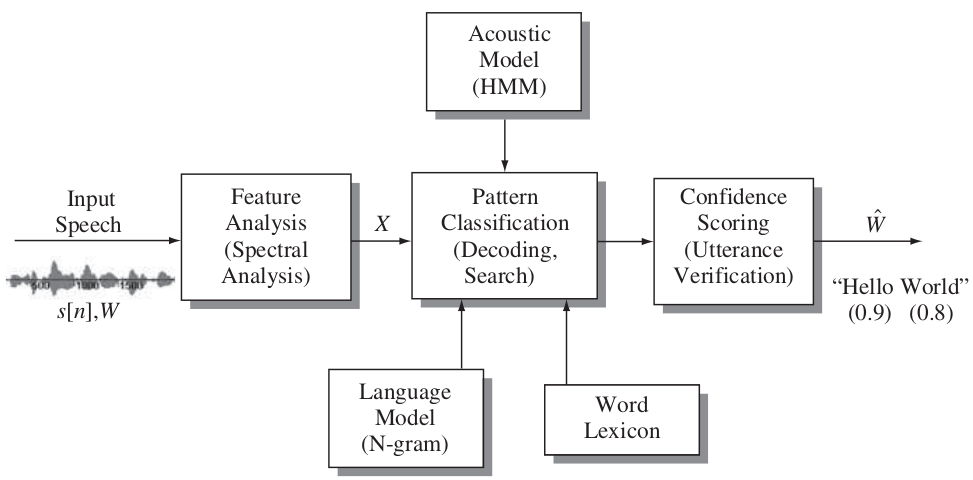
\includegraphics[width=0.6\textwidth]{ASR_diagram}
\end{figure}


\textbf{Mel Frequency Cepstral Coefficients}

Η πληροφορία του αρχικού σήματος φωνής $s[n]$ θα πρέπει να κωδικοποιηθεί κατάλληλα έτσι ώστε να δωθεί σαν είσοδο στο σύστημα αναγνώρισης προτύπων. Με φασματική ανάλυση το $s[n]$ μετατρέπεται σε ακολουθία διανυσμάτων χαρακτηριστικών \textbf{$X$} = \textbf{$(X_1,..,X_T)$}. Κάθε ένα απο τα $X_i$ αντιπροσωπεέυει τα χαρακτηριστικά για ένα παράθυρο του σήματος.

Τα πιο συνηθισμένα χαρακτηριστικά ειναι τα MFCCs. Τα χαρακτηριστικά αυτά προκύπτουν απο την συστοιχία φίλτρων MEL με εφαρμογή του DCT (Discrete Cosine Transform) για να εισαχθεί ανεξαρτησία. Η απαίτηση για ανεξάρτητα features απορέει απο την αδυναμία των περισσότερων αλγόριθμων εκμάθησης να αναγνωρίσουν περίπλοκες εξαρτήσεις, και για αυτό οδηγεί σε καλύτερα αποτελέσματα. Παρουσιάζουμε τα στάδια υπολογισμού των MFCCs:

\textbf{Pre-emphasis}: Η διαδικασία προ-επεξεργασίας του σήματος γίνεται για κανονικοποίηση συχνοτήτων, μερική αποθορυβοποίηση αλλα και numerical stabillity. Εφαρμόζεται το φίλτρο $y(t) = x(t) - α\cdot x(t-1)$ όπου $α$ κατάλληλος συντελεστής. Όπως βλέπουμε γίνεται smoothing του σήματος στον χρόνο. 

\textbf{Παραθυροποίηση}:  Η παραθυρωποίηση είναι απαραίτητη για να διατηρηθούν οι χρονικές εξαρτήσεις του σήματος. Εάν υπολογίζαμε τον μετασχηματισμό Fourier στο σύνολο του σήματος δεν θα μπορούσαμε τοπικά να διακρίνουμε το φασματικό περιεχόμενο. Χωρίζουμε το σήμα σε επικαλυπτόμενα πλαίσια και εφαρμόζουμε την συνάρτηση παραθύρου. Μια τέτοια συνάρτηση ειναι το παράθυρο Hamming: 

\begin{figure}[h]
\caption{Hamming Window (πηγή:[2])}
\centering
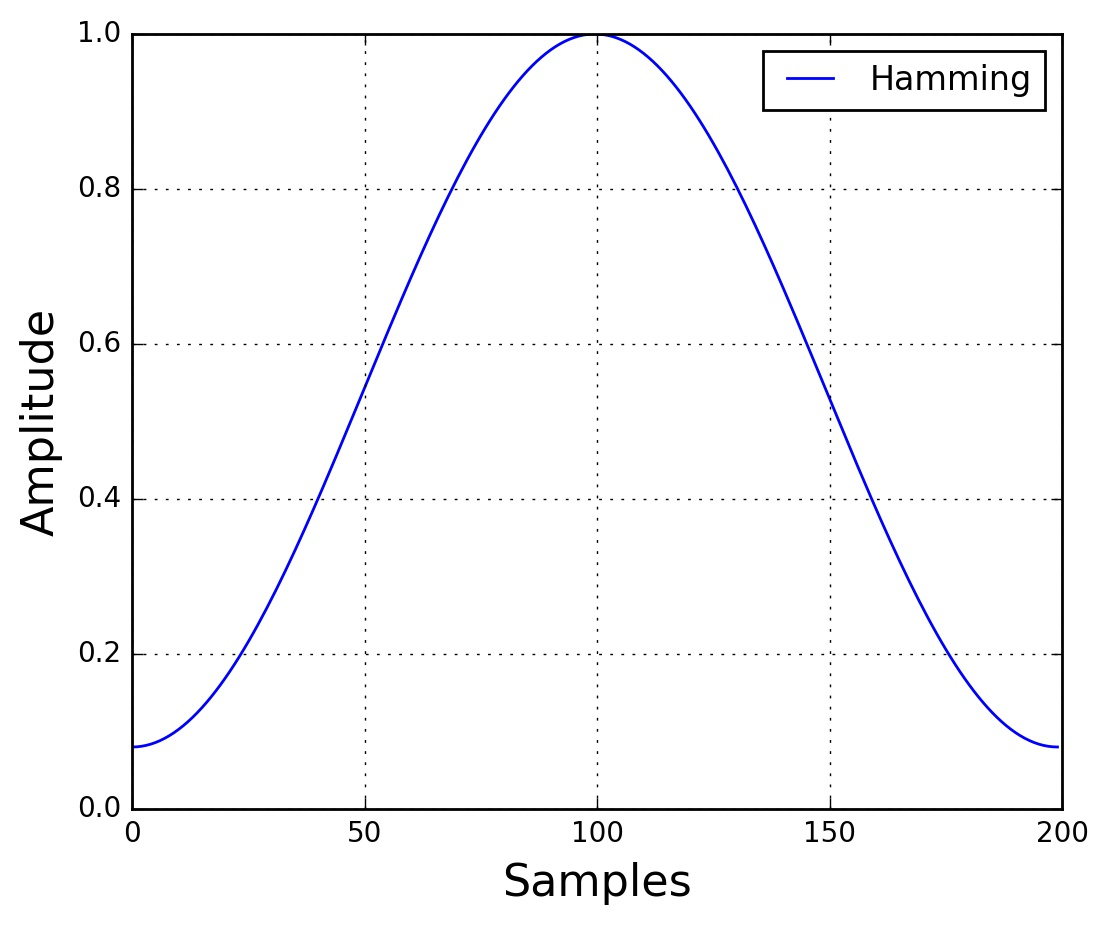
\includegraphics[width=0.4\textwidth]{hamming_window}
\end{figure}

\textbf{Fourier-Transform}: Υπολογίζοντας σε κάθε  παράθυρο τον FFT N-σημείων βρίσκουμε τον $STFT$ του σήματος. Ο $STFT$ μπορεί να μας δώσει μια εκτίμηση του φασματικού περιεχομένου στον χρόνο. Το φάσμα ισχύος μπορεί να υπολογιστεί απο την σχέση: 

$$P = \frac{|FFT(x_i)|}{N}$$ 
Όπου $N$ ο αριθμός των παραθύρων, και $FFT(X_i)$ ο FFT στο παράθυρο αριθμού $i=1,..,N$.  

\textbf{Mel Filterbanks}: Όπως έχουμε αναφέρει τα Mel Filterbanks έχουν σχεδιαστεί με γνώμονα ψυχοακουστικά μοντέλα απο έρευνα σε ανθρώπους. Έχουν ως σκοπό να μιμηθούν τον μή γραμμικό τρόπο που ο άνθρωπος αντιλαμβάνεται τον ήχο. Για τον λόγο αυτό έχουν τριγωνική μορφή και το τελικό φίλτρο προκύπτει όπως το παρακάτω σχήμα, δίνοντας περισσότερη έμφαση σε χαμηλές συχνότητες κοντά στο $0$ και λιγότερη σε υψηλές. Η κλίμακα mel μετατρέπει τις συχνότητες με βάση την ανθρώπινη αντίληψη:

$$m=2595\cdot log_{10}(1+\frac{f}{700})$$

Τα φίλτρα εφαρμόζονται στο φάσμα ισχύος (περιοδόγραμμα) του σήματος στην κλίμακα Mel. Συνήθως εφαρμόζονται 26 φίλτρα οπότε προκύπτουν και 26 συντελεστές. Τα τελικά MFC (Mel Filterbank Coefficients, χωρίς DCT) προκύπτουν λογαριθμίζοντας το αποτέλεσμα. Ο λογάριθμος μοντελοποιεί την ανθρώπινη αντίληψη για την ένταση του ήχου, που είναι κατα βάση λογαριθμική. 

\begin{figure}[h]
\caption{Η συστοιχία φίλτρων Mel σε κλίμακα mel (πηγή:[2])}
\centering
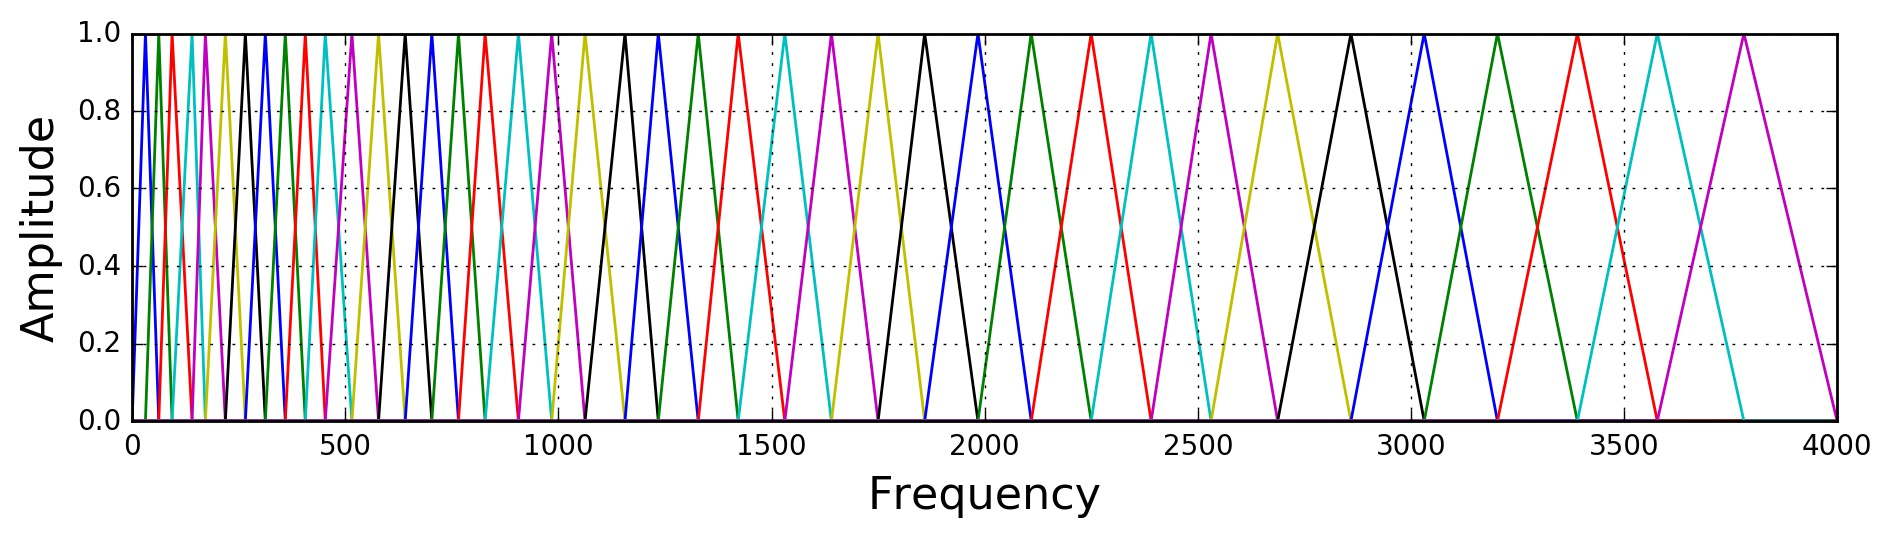
\includegraphics[width=0.6\textwidth]{mel_filters}
\end{figure}


\textbf{DCT και mean-normalization} Τα τελευταία βήματα αποσκοπούν στην δημιουργία ανεξάρτητων features. Πρέπει να σημειώσουμε οτι δεν έχουν σκοπό την εξαγωγή πληροφορίας με βάση την γνώση μας για τον άνθρωπο και την φύση του task, αλλα ειναι απαραίτητα για την εφαρμογή των αλγορίθμων εκμάθησης που θα εφαρμόσουμε στην συνέχεια. 

Ο μετασχημτισμός $DCT$ είναι γραμμικος και για αυτό χάνεται λίγη πληροφορία, οδηγεί όμως σε ανεξάρτητα feartures. Ουασιστικά το σήμα εκφράζεται σαν άθροισμα συνιμητόνων σε διαφορετικές συχνότητες. Η κανονικοποίηση εφαρμόζεται για αποθορυβοποίηση, και απαλοιφή του bias υπερ χαμηλών συχνοτήτων. 

Στην πράξη διατηρούντε οι συντελεστές $1-13$ ενώ μπορούν να ενταχθούν στο διάνυσμα χαρακτηριστικών και οι πρώτοι και δεύτεροι παράγωγοι των MFCCs.


\bigbreak
\bigbreak
\textbf{Γλωσσικά Μοντέλα (Language Models)}

Ένα γλωσσικό μοντέλο αντιστοιχίζει μια πιθανότητα σε κάθε πιθανή ακολουθία λέξεων. 

Τα γλωσσικά μοντέλα είναι απαραίτητα σε tasks αναγνώρισης φωνής γιατί προσφέρουν σημαντική πληροφορία για την κατανομή των λέξεων, διευκολύνοντας την αναγνώριση τους. Εάν ένας συγκεκριμένος συνδιασμός λέξεων σε μια πρόταση ειναι ελάχιστα πιθανός τότε μπορούμε να διαπιστώσουμε οτι έχει γίνει σφάλμα. Κάτι τέτοιο δε θα ήταν δυνατό αν εξετάζαμε τις λέξεις χωριστά. 

$$P(w_1,...,w_n) = P(w_1)P(w_2|w_1)...P(W_n|w_1...w_{n-1}) = \prod_{k=1}^nP(w_k|w_1..w_{k-1})$$

Άρα μπορούμε να υπολογίσουμε την πιθανότητα εμφάνισης της ακολουθίας υπολογίζοντας την πιθανότητα κάθε λέξης με δεδομένες τις προηγούμενες. Η απλοποίηση οτι μόνο οι n-1 προηγούμενες λέξεις έχουν σημασία οδηγεί σε $n-gram$ μοντέλα. Στην άσκηση αναπτύξαμε bigram και unigram language models.

bigram: $P(w_n|w_1..w_{n-1}) = P(w_n|w_{n-1})$\\
Unigram: $P(w_n|w_1..w_{n-1}) = P(w_n)$

Οι πιθανότητες υπολογίζονται απο τα δεδομένα με μία MLE προσέγγιση (Maximum Likelihood Estimation). Η εκτίμηση ειναι MLE γιατί η συγκεκριμένη επιλογή για την πιθανότητα οδηγεί σε μεγιστοποίηση της πιθανοφάνεις του συνόλου δεδομένων $X_{train}$ .  Για ένα $n-gram$ μοντέλο η πιθανότητα εμφάνισης μίας ακολουθίας μπορεί να υπολογιστεί απο το corpus ως η σχετική συχνότηα εμφάνισης. Συμβολίζουμε με $C(s)$ τον αριθμό εμφανίσεων μιας ακολουθίας. 

$$ P(w_n|s) = \frac{C(s\cdot w_n)}{s}$$
Όπου $s = w_{n-1}...w_{n-N+1}$. 

\bigbreak
\bigbreak
\textbf{Φωνητικά Μοντέλα (Acoustic Models)}

Τα ακουστικά μοντέλα χρησιμοποιούντε για να αναπαραστήσουν την σχέση μεταξύ του σήματος εισόδου και των φωνημάτων ή λέξεων (ακουστικές μονάδες αναγνώρισης). Το μοντέλο  εκπαιδεύεται σε ένα σύνολο σημάτων φωνής για τα οποία κατέχουμε την μεταγραφή (transcription) και κατάλληλα διάσπαση στις μονάδες αναγνώρισης με labels. Έτσι μπορέι να δημιουργήσει μια στατιστική αναπαράσταση για κάθε κατάσταση του μοντέλου.

Τα πιο διαδεμονένα μοντέλα είναι τα HMM (Hidden Markov Models). Έστω οτι παρατηρούμε  μια ακολουθία $\textbf{x}$, σε κάθε μία τις παρατηρηήσεις $o_i$ αντιστοιχίζουμε μια κρυφή μεταβλητή (latent variable) $q_i$. Οι $q_i$ σχηματίζουν αλυσίδα Markov, δηλαδή  $P(q_n|q_{n-1},q_{n-2},..) = P(q_n|q_{n-1})$. Οι παράμετροι του μοντέλου ειναι ο πίνακας μετάβασης $\textbf{A}= a_{ij}$ απο την κατάσταση $i$ στην $j$, η αρχική κατανομή $\textbf{π}$, και οι πιθανότητες παρατήρησης της ακολουθίας που συμβολίζουμε $B = \{b_j(o_i)\}$ όπου κάθε μια αναπαριστά την πιθανότητα η παρατήρηση $o_i$ να έχει παραχθεί απο την κατάσταση $j$ . Η τελευταία συνδέει την παρατηρούμενη ακολουθία με τις κρυφές μεταβλητές και λέγεται emission probability.  Σε μοντέλα φωνής η κατανομή είναι συνήθως μίξη Γκαουσιανών, και η αλυσίδα αρχίζει απο την $q_1$ πηγαίνοντας μόνο προς τα μπροστά. 

Η εκτίμηση των παραμέτρων $(A,B,π) $ της βέλτιστης αντιστοίχισης μεταξύ καταστάσεων του μοντέλου και της ακολουθίας ειδόδου γίνεται επαναληπτικά βελτιώνοντας κάθε φορά την πιθανοφάνεια (Forward-Backward Algorithm). Ένα $HMM$ μπορεί να εκπαιδευτεί για την αναγνώριση ενός φωνήματος και με τον forward αλγόριθμο να υπλογιστεί η πιθανότητα $P(\textbf{x}|λ)$,  όπου $λ = (A,B,π)$ το μαρκοβιανό μοντέλο. Υπολογίζεται δηλαδή πόσο πιθανή ειναι η ακολουθία σύμφωνα με το μοντέλο. Σαν είσοδο δίνουμε κατάλληλο feature vector όπως $MFCCs$.

Δημιουργώντας μοντέλα αναγνώρισης φωνημάτων και συνδέοντας τα μπορούμε να δημιουργήσουμε μοντέλα αναγνώρισης λέξεων και προτάσεων. Η state-of-the-art τεχνική είναι η χρήση triphones, δηλαδή τριάδας φωνημάτων εισάγοντας πληροφορία context.


\begin{figure}[h!]
\caption{HMM μοντέλο}
\centering
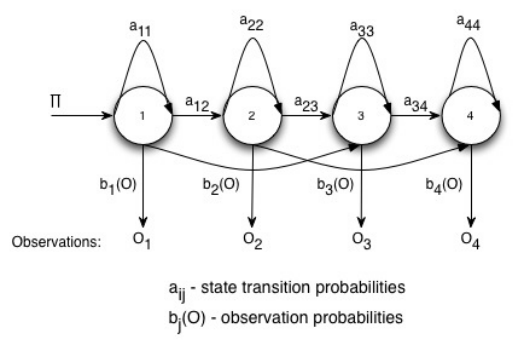
\includegraphics[width=0.65\textwidth]{hmm1.png}
\end{figure}

\pagebreak

\subsection*{Βήμα 3}
Σε αυτό το βήμα αρχικά, δημιουργήσαμε τον φάκελο data και μέσα σε αυτόν τους φακέλους train, dev και test. Σε κάθε ένα από αυτούς τους φακέλους δημιουργήσαμε με τη χρήση regular expressions τα εξής αρχεία: 
\begin{itemize}
    \item \textbf{uttids:} περιέχει στην κάθε του γραμμή ένα μοναδικό συμβολικό όνομα για κάθε πρόταση του συγκεκριμένου συνόλου δεδομένων δηλαδή δημιουργήσαμε τα  utterance-ids
    \item \textbf{utt2spk:} περιέχει σε κάθε γραμμή τον ομιλητή που αντιστοιχεί σε κάθε πρόταση και είναι της μορφής: utterance-id-1 speaker-id. Ως speaker-id επιλέξαμε αντίστοιχα τα m1, m3, f1, f5.  
    \item \textbf{wav.scp:} περιέχει τη θέση του αρχείου ήχου που αντιστοιχεί σε κάθε πρόταση και είναι της μορφής: utterance-id-1 /path/to/wav1 .
    \item \textbf{text:} περιέχει το κείμενο που αντιστοιχεί στην κάθε πρόταση και είναι της μορφής: utterance-id-1 utterance-id-2 κ.ο.κ.
\end{itemize}
Αφού δημιουργήσαμε αυτά τα αρχεία, αντικαταστήσαμε σε κάθε αρχείο text τις προτάσεις με τις αντίστοιχες αλληλουχίες φωνημάτων χρησιμοποιώντας το αρχείο lexicon.txt το οποίο αντιστοιχίζει κάθε λέξη με της αγγλικής γλώσσας με την αλληλουχία φωνημάτων της. Ακόμα, στην αρχή και στο τέλος κάθε πρότασης προσθέσαμε το φώνημα sil της σιωπής.
Για να δημιουργηθεί το αρχείο text αφαιρέσαμε τους ειδικούς χαρακτήρες εκτός από τα μονά εισαγωγικά και κάναμε όλα τα γράμματα μικρά. Η διαδικασία για την δημιουργία αυτών των αρχείων και των φακέλων φαίνεται στον python κώδικα Step\_3\_4.1.py.

\subsection*{Βήμα 4.1}
Σε αυτό το βήμα δημιουργήσαμε τα directories που θα χρειαστούμε για την υλοποίηση της άσκησης με βάση τα directories της Wall Street Journal όπως φαίνεται στην παρακάτω εικόνα. 

\begin{figure}[h]
\caption{Δομή φακέλων για το Kaldi (πηγή:[4])}
\centering
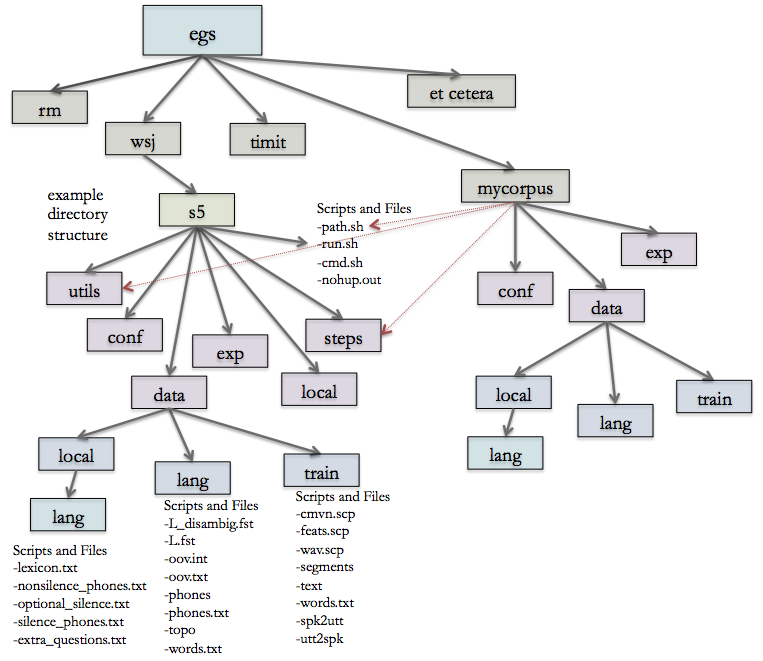
\includegraphics[width=0.6\textwidth]{directorystructure2.png}
\end{figure}

Αρχικά, δημιουργήσαμε τους φακέλους usc και μέσα σε αυτόν τον φάκελο s5 στον οποίο βάλαμε τον φάκελο data που δημιουργήσαμε στο προηγούμενο βήμα.
Στη συνέχεια, από τη διαδικασία για τη Wall Street Journal που βρίσκεται στο φάκελο egs αντιγράψαμε  τα αρχεία path.sh και cmd.sh στο δικό μας directory. Επειδή κρατήσαμε την ίδια δομή φακέλων με την WSJ δεν χρειάστηκε να αλλάξουμε το path του Kaldi όμως, χρειάστηκε να αλλάξουμε τις μεταβλητές train\_cmd, decode\_cmd και cuda\_cmd από queue.pl σε run.pl έτσι ώστε ο κώδικας που έχουμε γράψει να τρέχει τοπικά στον υπολογιστή μας και όχι να κάνουμε allocate machines χρησιμοποιώντας Sun Grid Engine.
Ακόμα, από την WSJ χρειάστηκε να πάρουμε τους φακέλους steps και utils για αυτό δημιουργήσαμε soft links με την εντολή ln -s file1 link1 στον ίδιο φάκελο με αυτόν την WSJ.
Τέλος, δημιουργήσαμε τους φακέλους conf, data/lang και data/local/dict, data/local/lm\_tmp, data/local/nist\_lm όπως φαίνεται και στην παραπάνω εικόνα.
Για να δημιουργήσουμε τα links και τα directories αυτού του βήματος τρέξαμε τον κώδικα Step\_3\_4.1.py.

\subsection*{Βήμα 4.2}
\textbf{Βήμα 4.2.1}

Σε αυτό το βήμα έγινε η προετοιμασία του γλωσσικού μοντέλου. 
Αρχικά, μέσα στον φάκελο data/local/dict δημιουργήσαμε και αποθηκεύσαμε τα εξής αρχεία:
\begin{itemize}
    \item \textbf{silence\_phones.txt} και \textbf{optional\_silence.txt} που περιέχουν μόνο το φώνημα της σιωπής (sil).
    \item \textbf{nonsilence\_phones.txt} το οποίο περιέχει όλα τα υπόλοιπα φωνήματα. Τα φωνήματα είναι sorted και είναι ένα σε κάθε γραμμή του αρχείου.
    \item \textbf{lexicon.txt} το οποίο αντιστοιχίζει κάθε φώνημα στον εαυτό του. Κάθε γραμμή του αρχείου έχει την εξής μορφή: sil sil φωνήμα1 φώνημα1 φώνημα2 φώνημα2 κοκ.
    \item \textbf{lm\_train.text, lm\_test.text και lm\_dev.text} τα οποία είναι ίδια με τα αντιστοιχα αρχεία text με τη διαφορά ότι στην αρχή της πρότασης προσθέσαμε το σύμβολο <s> και στο τέλος το </s>.
    \item \textbf{extra\_questions.txt} το οποίο είναι κενό.
\end{itemize}
Τα αρχεία αυτά δημιουργήθηκαν εκτελώντας τον python κώδικα Step\_4.2.1.py.

\textbf{Βήμα 4.2.2}

Σε αυτό το βήμα δημιουργήσαμε την ενδιάμεση μορφή του γλωσσικού μοντέλου.
Για αυτό το σκοπό χρησιμοποιήσαμε την εντολή build-lm.sh του πακέτου IRSTLM που έχει εγκατασταθεί μαζί με το Kaldi. 
Για το unigram μοντέλο καλέσαμε την εντολή:

\$KALDI\_ROOT/tools/irstlm/scripts/build-lm.sh -i data/local/dict/lm\_train.text -n 2 -o data/local/lm\_tmp/lm\_train\_unigram.ilm.gz

Ενώ για το bigram την εντολή: 

\$KALDI\_ROOT/tools/irstlm/scripts/build-lm.sh -i data/local/dict/lm\_train.text -n 1 -o data/local/lm\_tmp/lm\_train\_unigram.ilm.gz.

\textbf{Βήμα 4.2.3}

Σε αυτό το βήμα κάναμε compile το γλωσσικό μοντέλο και το αποθηκεύσαμε στον φάκελο data/local/nist\_lm σε μορφή ARPA. Η εντολή που χρησιμοποιήθηκε είναι η 

compile-lm <αρχείο.ilm.gz> -t=yes /dev/stdout | grep -v unk | gzip -c > <αρχειο\_εξόδου.arpa.gz>.

\textbf{Βήμα 4.2.4}

Σε αυτό το βήμα δημιουργήσαμε το λεξικό της γλώσσας L.fst χρησιμοποιώντας την εντολή του Kaldi 

./utils/prepare\_lang.sh data/local/dict "<oov>" data/local/lang data/lang. 

Το δεύτερο όρισμα “<oov>” αναφέρεται σε κάποιο φώνημα που υποδεικνύει το φώνημα της σιωπής ή σε κάποιο φώνημα που δεν είναι στο λεξικό “out of vocabulary”. Το όρισμα <oov> θα πρέπει να μπει στο λεξικό ως εξής <oov> <oov> καθώς και να μπει και στο αρχείο silence\_phones.txt. Σε παλαιότερες εκδόσεις του Kaldi τα source και tmp directories μπορούσαν να είναι τα ίδια όμως για την έκδοση που έχουμε πρέπει να δείχνουν σε διαφορετικούς φακέλους.

\textbf{Βήμα 4.2.5}

Σε αυτό το βήμα δημιουργήσαμε τη γραμματική των γλωσσικών μοντέλων G.fst. Για να δημιουργήσουμε αυτό το αρχείο, τροποποιήσαμε το αρχείο timit\_format\_data.sh που βρίσκεται στον φάκελο
./kaldi/egs/timit/s5/local/.
Από το αρχείο αυτό κρατήσαμε μόνο τη δημιουργία των directories καθώς και την εντολή που δημιουργεί το G.fst. Η εντολή αυτή είναι η εξής: 

gunzip -c path\_to/lm\_train.arpa.gz |  arpa2fst --disambig-symbol=\#0 --read-symbol-table=
path\_to/words.txt - data/lang\_test/G.fst .

Η εντολή αυτή παίρνει ένα αρχείο .arpa.gz και το μετατρέπει σε .fst. Την εντολή την καλέσαμε δύο φορές μία για το unigram γλωσσικό μοντέλο και μία για το bigram στα δεδομένα του train.
Ο κώδικας για τα παραπάνω βήματα βρίσκεται στο bash script Steps\_4.2.2-5.sh.

\textbf{Ερώτημα 1}

Ενα χαρακτηριστικό του γλωσσικού μοντέλου για μία συγκεκριμένη εφαρμογή (task) είναι το $\text{Language Perplexity}$. Αποτελεί μία μετρική της πολυπλοκότητας του γλωσσικού μοντέλου και ορίζεται ως ο γεωμετρικός μέσος του μέσου αριθμού λέξεων που ακολουθούν μία τυχαία λέξη στο corpus (word-branching factor). Η εντροπία ορίζεται: 
$$ H(W) = -\sum P(W) log_2P(W)$$
Οπότε το perplexity για μία κατανομή μπορεί να οριστεί:

$$2^{H(p)} = 2^{-\sum P(W) log_2P(W)} $$.

Ο ρυθμός εντροπίας μιας στοχαστικής διαδικασίας ορίζεται: 
$$H(W) = -\frac{1}{M} H(W_1,W_2,...,W_M) = -\frac{1}{M} \sum p(W_1,...,W_M) log_2 p(W_1,...,W_M) , M \to \infty$$

Στο πλαίσιο ενός γλωσσικού μοντέλου είναι η εντροπία ανα λέξη. 
Για εργοδοτικές, στάσιμες διαδικασίες μπορεί να απλοποιηθεί στην σχέση:
$$H(W) = -\frac{1}{M} log_2 p(W_1,...,W_M) $$
Με την λογικη ότι καθώς $M \to \infty$ οι ιδιότητες του συνόλου αντιπροσωπεύονται επαρκώς απο μία μόνο ακολουθία. 
Το Language Perplexity μπορεί τώρα να οριστεί:

$$PP(W) = 2^{H(W)} = P(W_1,W_2,...,W_M)^{-1/M} , M \to \infty $$
$$PP(W) = \sqrt[M]{\frac{1}{P(W_1,W_2,...,W_M)}}$$

Για unigram μοντέλα η σχέση απλοποιείται σε: 
$$\sqrt[M]{\frac{1}{\prod_{i=1}^MP(W_i)}}$$
Και για bigram:
$$\sqrt[M]{\frac{1}{\prod_{i=1}^MP(W_i|W_{i-1})}}$$


Βλέπουμε λοιπόν οτι το perplexity είναι ο γεωμετρικός μέσος του αντιστρόφου της πιθανότητας που έχει ορίσει το μοντέλο μας για κάθε μια λέξη ή ακολουθία λέξεων. Η ρίζα χρησιμοποιείται για κανονικοποίηση στον αριθμό των λέξεων. Εαν το υπολογίσουμε πάνω στο test ή το validation set διαισθητικά έχουμε ένα μέτρο για το πόσο καλά μπορεί το μοντέλο μας να προβλέψει λέξεις πάνω στα σύνολα. Εάν οι πιθανότητες που τοποθετούνται στις λέξεις του συνόλου είναι υψηλές τότε το perplexity είναι χαμηλό και το μοντέλο περιγράφει καλά άγνωστες λέξεις.  Έχει δηλαδή μεγαλύτερη ακρίβεια. 

Συνεπώς για δύο μοντέλα που έχουν εκπαιδευτή στο train set με το ίδιο λεξιλόγιο, το perplexity ειναι μια καλή μετρική σύγκρισης της απόδοσης τους. Περιμένα οτι απο τα μοντέλα που εκπαιδεύσαμε το bigram θα έχει καλύτερη επίδοση απο το unigram και στα δύο σύνολα. Χρησημοποιώντας την εντολή του $Kaldi$ complile-lm υπολογίζουμε το perplexity πάνω στα dev, test sets για το γλωσσικό μοντέλο του train: 

\begin{center}
\begin{tabular}{ |c|c|c|c| } 
 \hline
    &Perplexity & Number of words & OOV\% \\
 \hline 
 Dev Unigram & 55.48 & 6540 & 2.80\\
\hline 
 Dev Bigram & 26.94 & 6540 & 2.80\\
\hline 
 Test Unigram & 55.39 & 6363 & 2.89\\
\hline 
 Test Bigram & 26.45 & 6363 & 2.89\\
\hline 
\end{tabular}
\end{center}

Τα αποτελέσματα είναι όπως περιμέναμε και παρόμοια στο Test και Dev set. 
Σημειώνουμε οτι η βελτίωση στο perplexity δεν ισοδυναμεί πάντα με βελτίωση στην ακρίβεια του μοντέλου. 



\subsection*{Βήμα 4.3}
Σε αυτό το βήμα έγινε η εξαγωγή των ακουστικών χαρακτηριστικών. Συγκεκριμένα, για κάθε ένα από τα sets train, test και dev εξαγάγαμε τα MFCCs  χρησιμοποιώντας τις εντολές του Kaldi make\_mfcc.sh, compute\_cmvn\_stats.sh. Η πρώτη εντολή κάνει extract τα MFCC ακουστικά χαρακτηριστικά ενώ η δεύτερη υπολογίζει cepstral mean και variance normalization (CMVN) στατιστικά. 


\subsection*{Ερώτημα 2}

Η τεχνική Cepstral mean and variance normalization (CMVN) χρησιμοποιείται για σταθερή (robust) αναγνώριση φωνής. Είναι μια υπολογιστικά αποδοτική τεχνική κανονικοποίησης. Χρησιμοποιείται για την αφαίρεση επιδράσεων καναλιού (περιβάλλον μετάδοσης, φωνητική όδος, κτλπ.). Παρ'όλα αυτά μπορεί να οδηγήσει και σε παραμόρφωση μειώνοντας την απόδοση σε περιβάλλοντα με χαμηλο SNR, και η κανονικοποίηση σε $μ=0, σ^2 =1$ αφαιρεί διακριτικά χαρακτηριστικά ανάμεσα στους συντελεστές. 

Έστω $x[n]$ το σήμα εισόδου φωνής, μπορούμε να μοντελοποιήσουμε τις επιδράσεις του καναλιού ως συνέλιξη με ένα φίλτρο απόκρισης $h[n]$. 

Τελικό σήμα: $y[n] = x[n] * h[n]$, και με FFT $Y[f] = X[f] H[f]$. Έπειτα παίρνουμε την ένεργεια του FFT και πολλαπλασιάζουμε με τα φίλτρα για να προκύψουν οι συντελεστές Mel:
$MF_[r] =  V_r[m]|X[m] H[m]|^2 $, όπου m στην κλίμακα mel, $V_r[m]$ το φίλτρο $r$. 

Λογαριθμίζουμε και οι όροι διαχωρίζονται:
$logMF_[r] =  log(V_r[m]|X[m]|^2) + 2log(|H[m]|) $. 

Ο DCT είναι γραμμική συνάρτηση άρα: $mfcc[r] =  \sum_i a_i log(V_r[m]|X[m]|^2) + \sum_i a_i 2log(|H[m]|)$. 

Παρατηρούμε τώρα ότι αν αφαιρέσουμε απο κάθε συντελεστή την μέση τιμή ο όρος $H[m]$ απαλοίφεται γιατί: $mfcc_{mean} = \sum_r \sum_i a_i log(V_r[m]|X[m]|^2)/R + \sum_i a_i 2log(|H[m]|)$. Δηλαδή η μέση τιμή περιέχει τον ίδιο όρο θορύβου με τα $mfccs$. Για προσθετικό θόρυβο δεν έχουμε βελτίωση. 

Στην πραγματικότητα όπως βλέπουμε απο το [1] η σχέση ειναι σημαντικά πιο πολύπλοκη: 
$$mfcc_m[n] = \frac{1}{R} \sum_{r=1}^R log(MF_m[r])cos[2π/R(r+1/2)^n]$$

όπου $MF_m[r] = \frac{1}{A_r} \sum_{k=L_r}^{U_r} |V_r[k] Y_m[k]|^2 , r \in{1,R}$. 
Τα MFs είναι το αποτέλεσμα της συστοιχίας Mel και τα Vr[k] τα αντίστοιχα φίλτρα, $m$ ο αριθμός παραθύρου, $A_r$ σταθερά κανονικοποίησης. 

Η γενική παρατήρηση ισχύει.

\subsection*{Ερώτημα 3}

Με τις εντολές του $Kaldi$ feat-to-dim, feat-to-len εξάγουμε για το x\_train των αριθμό των MFCCs και τον αριθμό των παραθύρων για  τις πρώτες 5 προτάσεις. Προκύπτουν 13 coefficients, που είναι και η συνηθισμένη επιλογή για τον αριθμό συντελεστών. Τα παράθυρα διαφέρουν προφανώς και εξαρτώνται απο το  μήκος του σήματος. 

\begin{center}
\begin{tabular}{ |c|c|c| } 
 \hline
    & Number of MFFCs & Number of Frames  \\
 \hline 
f1-usctimit-ema--184 & 13 & 237\\  \hline 
f1-usctimit-ema--185 & 13 & 377 \\  \hline 
f1-usctimit-ema--186 & 13 & 317 \\  \hline 
f1-usctimit-ema--187 & 13 & 399 \\  \hline 
f1-usctimit-ema--188 & 13 & 338\\  \hline 
\end{tabular}
\end{center}


\subsection*{Βήμα 4.4}
Σε αυτό το βήμα εκπαιδεύσαμε τα ακουστικά μοντέλα και αποκωδικοποιήσαμε τις προτάσεις.

\textbf{Βήμα 4.4.1}

Εκπαιδεύσαμε ένα monphone GMM-HMM ακουστικό μοντέλο πάνω στα train δεδομένα. Επειδή αρχικά δεν έχουμε εκπαιδεύσει κάποιο μοντέλο δεν υπάρχει κάποιο source directory και άρα στην παρακάτω εντολή το source και το destination directory είναι το ίδιο. Η εντολή που χρησιμοποιήσαμε είναι η εξής: 

./steps/train\_mono.sh --boost-silence 1.25 –nj 4 --cmd "run.pl" ./data/train ./data/lang\_test ./exp/mono

To --nj 4 είναι για το πόσα jobs μπορούν να γίνουν παράλληλα. Το Kaldi όταν βάζουμε στην εντολή αυτή την επιλογή χωρίζει τα δεδομένα σε 4 τμήματα και κρατάει τα δεδομένα για τους ίδιους ομιλητές μαζί. Βάζουμε λοιπόν το 4  στην μεταβλητή nj γιατί έχουμε 4 ομιλητές στην άσκηση.  Ακόμα, η επιλογή - - boost-silence είναι ένα standard πρωτόκολλο για το training του μοντέλου μας.

\textbf{Βήμα 4.4.2}

Σε αυτό το βήμα δημιουργήσαμε τον γράφο HCLG του Kaldi σύμφωνα με τη γραμματική G.fst. 
Δημιουργούμε δύο γράφους για τα train δεδομένα έναν για το unigram γλωσσικό μοντέλο και ένα για το bigram. Για τη δημιουργία του γράφου χρησιμοποιήσαμε την εντολή 

./utils/mkgraph.sh --mono ./data/lang\_test ./exp/mono exp/mono/graph\_x όπου το x είναι ή unigram ή bigram.

\textbf{Βήμα 4.4.3}

Στο βήμα αυτό χρησιμοποιήσαμε το script decode.sh του kaldi για να αποκωδικοποιήσουμε τις προτάσεις των validation και test δεδομένων για το unigram και το bigram γλωσσικό μοντέλο.
Η εντολή που εκτελέσαμε είναι η παρακάτω: 

./steps/decode.sh exp/mono/graph\_\$y ./data/\$x ./exp/mono/decode\_\${x}\_\${y} 
,όπου το x παίρνει τις τιμές test και dev και το y τις τιμές unigram και bigram.

Η εντολή αυτή καλεί το script ./local/score.sh του Kaldi το οποίο δεχεται τις παραμέτρους  --min-lmwt και --max-lmwt για το ελάχιστο και μέγιστο βάρος του γλωσσικού μοντέλου. Με βάση αυτά τυπώνει στα αρχεία wer\_N το PER για κάθε διαφορετικό βάρος.
Το βάρος του γλωσσικού μοντέλου είναι δίνει περισσότερη βαρύτητα  αντίστοιχα στα γλωσσικά μοντέλα ή στα ηχητικά σήματα.
Η εύρεση του καλύτερου score γίνεται ανοίγοντας όλα τα lattice αρχεία και παίρνοντας από αυτά τις καλύτερες τιμές για τα φωνήματα σε όλα τα utterances τα οποία περιέχουν. Η καλύτερη τιμή δίνεται από την 
<kalid-trunk>/src/latticebin/lattice-best-path<kalid-trunk>/src/latticebin/lattice-best-path
και το language model weight δίνεται μέσω της -lm-scale.

Τέλος, το PER υπολογίζεται χρησιμοποιώντας την 
<kalid-trunk>/src/bin/computer-wer<kalid-trunk>/src/bin/computer-wer, 
η οποία παίρνει δύο transcription files (την καλύτερη τιμή που έδωσε το lattice στο προηγούμενο βήμα και τα σωστά labels ) και δίνει την καλύτερη τιμή για το συγκεκριμένο γλωσσικό μοντέλο και για όλα τα language model weights. 

\textbf{Βήμα 4.4.4}

Μετά την εκτέλεση της παραπάνω εντολής  έχουμε στους φακέλους ./exp/mono/decode\_\${x}\_\${y} με x και y τα παραπάνω, τα wer αποτελέσματα για τα test και train δεδομένα και για το unigram και bigram μοντέλο. Στην δική μας άσκηση το WER ταυτίζεται με το PER που θέλουμε αφού σαν λέξη (Word Error Rate) θεωρείται το κάθε φώνημα (Phone Error Rate).

Τα αποτελέσματα φαίνονται παρακάτω.

\begin{center}
\begin{tabular}{ |c|c|c|c|c|c| } 
 \hline
    &PER\% & INS & DEL & SUB & lmwt\\
 \hline 
 Dev Unigram & 51.96 & 81 & 1725 & 1402 & 7\_0.0 \\
\hline 
 Dev Bigram & 51.96 & 81 & 1725 & 1402 & 7\_0.0 \\
\hline 
 Test Unigram & 50.03 & 48 & 1638 & 1313 & 7\_0.0\\
\hline 
 Test Bigram & 50.03 & 48 & 1638 & 1313 & 7\_0.0\\
\hline 
\end{tabular}
\end{center}

Παρατηρούμε ότι το καλύτερο αποτέλεσμα το έχουμε για το test set και οτι δεν έπαιξε ρόλο η unigram και bigram υλοποίηση για το G.fst. 

Οι δύο \textbf{υπερπαράμετροι της διαδικασίας scoring} σε αυτό το βήμα είναι οι \textbf{min max LM weights για lattice rescoring}. Αυτές οι μεταβλητές δείχνουν το βάρος στους λογάριθμους των πιθανοτήτων των γλωσσικών μοντέλων σε σχεση με τους λογαρίθμους των πιθανοτήτων των ακουστικών μοντέλων. Είναι ένας παράγοντας που αντισταθμίζει το υψηλό correlation των frames. Στο καλύτερο μας μοντέλο το οποίο είναι το test αυτές οι μεταβλητές πήραν τις τιμές 7 και 17 αντίστοιχα ενώ το καλύτερο PER το πήραμε για την τιμή 7.

\textbf{Βήμα 4.4.5}

Σε αυτό το βήμα κάναμε αρχικά align τα φωνήματα χρησιμοποιώντας το monophone μοντέλο και στη συνέχεια χρησιμοποιώντας αυτά τα alignments εκπαιδεύσαμε ένα triphone μοντέλο ακολουθώντας την ίδια διαδικασία με το monophone μοντέλο.
Για να κάνουμε το training χρησιμοποιήσαμε την παρακάτω εντολή:

./steps/train\_deltas.sh --boost-silence 1.25 2000 10000 ./data/train ./data/lang ./exp/mono\_ali ./exp/tri1 || exit 1;

Η εκπαίδευση του triphone μοντέλου περιλαμβάνει πρόσθετα arguments στην εντολή για τον αριθμό των leaves ή των καταστάσεων του HMM στο decision tree και για τον αριθμό των Gausssians. Στην παραπάνω εντολή λοιπόν καθορίσαμε 2000 HMM states και 10000 Gaussians. Αυτό σημαίνει ότι αν για παράδειγμα υπάρχουν 50 φωνήματα στο λεξικό μας θα μπορούσαμε να έχουμε μία κατάσταση HMM ανά φώνημα. Γνωρίζουμε όμως ότι τα φωνήματα διαφέρουν σημαντικά με ανάλογα με το αν βρίσκονται στην αρχή ή στο τέλος ή στη μέση μιας λέξης. Επομένως, θέλαμε τουλάχιστον τρεις διαφορετικές HMM καταστάσεις για κάθε φώνημα και άρα 150 καταστάσεις για όλα τα φωνήματα. Επιλέγοντας λοιπόν 2000 HMM καταστάσεις το μοντέλο μπορεί να αποφασίσει αν είναι καλύτερο να κατανείμει μία μοναδική κατάσταση σε πιο refined allophones του αρχικού φωνήματος. Αυτός ο διαχωρισμός των φωνημάτων αποφασίζεται από τις φωνητικές ερωτήσεις στο αρχείο questions.txt και extra\_questions.txt. Τα allophones αναφέρονται επίσης ως subphones, senones, HMM states, or leaves.

Ο ακριβής αριθμός φύλλων και Gaussians συχνά αποφασίζεται με βάσει κάποιων ευριστικών τιμών. Οι αριθμοί αυτοί εξαρτώνται σε μεγάλο βαθμό από την ποσότητα των δεδομένων, τον αριθμό των φωνητικών ερωτήσεων και τον στόχο του μοντέλου. Ο αριθμός των Gaussians δεν θα πρέπει να υπερβαίνει τον αριθμό των φύλλων. Οι αριθμοί αυτοί αυξάνονται αν συνεχίσουμε να βελτιώνουμε το μοντέλο μας με αλγορίθμους περαιτέρω εκπαίδευσης.

Τα αποτελέσματα του βήματος αυτού φαίνονται παρακάτω.

\begin{center}
\begin{tabular}{ |c|c|c|c|c|c| } 
 \hline
    &PER\% & INS & DEL & SUB & lmwt\\
 \hline 
 Dev Unigram & 37.63 & 264 & 752 & 1307 & 7\_0.0\\
\hline 
 Dev Bigram & 37.63 & 264 & 752 & 1307 & 7\_0.0\\
\hline 
 Test Unigram & 36.07 & 181 & 811 & 1208 & 8\_0.0\\
\hline 
 Test Bigram & 36.07 & 181 & 811 & 1208 & 8\_0.0\\
\hline 
\end{tabular}
\end{center}

Παρατηρούμε ότι το PER σε αυτή την περίπτωση μειώνεται και για τα δύο γλωσσικά μοντέλα (unigram, bigram). Και πάλι έχουμε την καλύτερη τιμή για το test set και τα unigram και bigram δεν επηρεάζουν το αποτέλεσμα. Σε αυτή την περίπτωση το lmwt παίρνει την τιμή 8\_0.0 για το test set.

Για την υλοποίηση των παραπάνω βημάτων τρέξαμε το script Step\_4.4.sh 

Τα αποτελέσματα από την εκτέλεση όλων των .py και .sh scripts φαίνονται στο .ipynb αρχείο με όνομα lab2.ipynb.


\textbf{Ερώτημα 4}

Είδη αναφερθήκαμε σε κρυφά μαρκοβιανά μοντέλα. Ένα HMM-GMM είναι ενα μαρκοβιανό μοντέλο $λ = (Α,B)$ ( η αρχική κατάσταση είναι η $q_1$) όπου $b_j = \sum_{m=1}^M c_{jm} \mathcal{N}(ο;μ_{jm}. Σ_{jm}), \sum c = 1$. Δηλαδή η πιθανότητα η παρατήρηση $ο_i$ να έχει δημιουργηθεί απο την κατάσταση j μοντελοποιείται απο βεβαρημένο άθροισμα (μίγμα) Γκαουσιαών. Το μαρκοβιανό μοντέλο κινείται απο αριστερά προς τα δεξιά και μία κατάσταση την φορά ή δεν κινείται: $a_{ij} = 0, j \neq i+1,i$. Εαν οι καταστάσεις αναπαριστούν φωνήματα η επανάληψη επιτρέπει σε ένα φώνημα να αναγνωριστεί 2 φορές. 

Ο ρόλος του $HMM$ είναι να εξάγει την πιθανότητα $P(O|λ)$ δηλαδή πόσο πιθανή είναι η ακολουθία με δεδομένο το μοντέλο. Αυτο το πετυχαίνει αντιστοιχίζοντας πλαίσια της ακολουθίας με καταστάσεις παρσάροντας ουσιαστικά το διάνυσμα χαρακτηριστικών $O$ σαν αυτόματο με τυχαίες μεταβάσεις μέσω του $A$. Η σχέση μεταξύ $o_i$ και καταστάσεων μοντελοποιειαι απο το $HMM$ σαν $GMM$. 

Η εκπαίδευση του μοντέλου γίνεται με τον Forward-Backward αλγόριθμο ή Naum-Welch. Συγκριμένα σε κάθε επανάληψη για όλο το συνόλο δεδομένων γίνεται αντιστοιχιση των πλαισίων με καταστάσεις του $HMM$. Για την βέλτιστη αντιστοίχιση υπολογίζονται εκτιμήσεις για τις $μ_{jm},σ_{jm}^2,c_{jm}$ με βάση τις προηγούμενες τιμές τους έτσι ώστε να μεγαλώνει η πιθανοφάνεια. Ο αλγόριθμος επαναλμβάνεται μέχρι να επιτευχθεί η ζητούμενη σύγκλιση.  Ο αλγόριθμος ειναι ουσιατικά $Ε-M$ (Expectation Maximization).  


\textbf{Ερώτημα 5}

Θα μοντελοποιήσουμε το πρόβλημα αναγνώρισης φωνής σαν στατιστικό πρόβλημα απόφασης. Συγκεκριμένα η πιο πιθανή λέξη (ή φώνημα) $\hat{W}$ δεδομένης μίας ακολουθίας χαρακτηριστικών $X$, είναι η $MAP$ (Maximum A Posteriori) εκτίμηση, δηλαδή αυτή που μεγιστοποιεί την a posteriori πιθανότητα. 
\begin{itemize}
    \item Το λεξικό
    \item Το γλωσσικό μοντέλο  
    \item Το ακουστικό μοντέλο
\end{itemize}
Ισχυεί:
$$ \hat{W} = arg max_W P(W|X) = arg max_W \frac{P(X|W)P(W)}{P(X)} = arg max_W P(X|W)P(W) $$  

Η a priori πιθανότητα της λέξης $P(W)$ θα προέλθει απο το γλωσσικό μοντέλο πάνω στο σύνολο λέξεων $X\_train$ ως εκτίμση της σχετικής συχνότητας. Ο όρος $P(X|W)$ αφορά το ακουστικό μοντέλο και υπολογίζεται απο την ανάλυση του $X$ με $HMM$ για την κάθε λέξη.  Η αναζήτηση γίνεται πάνω στο σύνολο όλων των λέξεων που ορίζεται απο το λεξικό. 

Έχοντας υλοποιήσει το διάνυσμα χαρακτηριστικών $X$ το ακουστικό μοντέλο θα υπολογίσει για κάθε κατάσταση $q$ του $HMM$ την πιθανοφάνεια του $x \in X$,  $p(x|q)$ με δεδομένη γλωσσική μονάδα, όπως φώνημα. Για να υπολογίσουμε την πιθανότητα χρησιμοποιούμε $GMM$. Το αποτέλεσμα είναι για κάθε παράθυρο ένα διάνυσμα που περιέχει την πιθανότητα να αντιστοιχεί σε αυτο κάθε φώνημα. Με χρήση του λεξικού που περιέχει την ανάλυση λέξεων σε φωνήματα υπολογίζουμε την πιθανότητα $P(X|W)$. Συνδιάζουμε με το language model όπως παραπάνω για την τελική εκτίμηση. Στην φάση του Decoding κάθε λέξη είναι ένα $HMM$ όπου τα φωνήματα είναι καταστάσεις ή σύνολα καταστάσεων. Για την γρήγορη αναζήτηση στα μοντέλα χρησιμοπιείται ο αλγόριθμος Viterbi.



\textbf{Ερώτημα 6}

Περιγράφουμε την δομή του γράφου $HCLG$ του $kaldi$:
\begin{itemize}
    \item Το $L.fst$ αντιστοιχίζει φωνήματα σε λέξεις. Σαν είδοσος στο fst δίνεται ακολουθία φωνημάτων και ακολουθώντας τις μεταβάσεις παίρνουμε σαν έξοδο την αντίστοιχει λέξη. 
    \item Το $G.fst$ είναι το γλωσσικό μοντέλο πάνω στις λέξεις του συνόλου δεδομένων (n-gram).
    \item Το $C.fst$ επεκτείνει τα φωνήματα σε context-dependent φωνήματα. Αντιστοιχίζει $tri-phones$ σε $mono-phones$
    \item Το $Η.fst$ αντιστοιχίζει πολλαπλές καταστάσεις $HMM$ σε triphones, έχει σαν input trainsition-ids (pdf-id και άλλες πληροφοριες). 
\end{itemize}

Ο συνολικός γράφος αποκωδικοποίησης (HCLG) αναπαριστά το γλωσσικό μοντέλο, το λεξικό με την αντιστοίχιση λέξεων σε φωνήματα, την πληροφορία συμφραζόμενων, και το HMM. Αποτελεί ένα fst που δέχεται $word-ids$ και επιστρέφει pdf-ids (αντιστοιχουν σε μοντέλα GMM). Για να είναι ο γράφος ντετερμινσιτικός εισάγονται disambiguation symbols.

\textbf{Model Optimizations}

\begin{itemize}
    \item Τα γλωσσικά μοντέλα παρουσιάζουν πρόβλημα όταν στο test set μπορεί να συναντήσουμε λέξεις που γνωρίζουμε την ύπαρξη τους, αλλα δεν έχουν εντοπιστεί στο συγκεκριμένο context (για παράδειγμα μετά απο μια άγνωστη λέξη). Στις λέξεις αυτές αντιστοιχίζεται μηδενική πιθανότητα. Για να το αποφύγουμε αυτο θα πρέπει να μειώσουμε την πιθανότητα άλλων γεγονότων και να την δώσουμε σε αυτά τα γεγονότα. Οι τεχνικές αυτές λέγονται smoothing ή discounting, και μπορεί να βελτιώσουν τα γλωσσικά μοντέλα μας. Αναλυτικά στο [3].
    \item Τα tri-phones εντοπίζονται σε state-of-the-art συστήματα επεξεργασίας φωνής. Θα μπορούσαμε όμως να κωδικοποιήσουμε περισσότερη πληροφορία συμφραζόμενων με χρήση n-phone μοντέλων (με κόστος αύξηση της υπολογιστικής πολυπλοκότητας).
    \item Σε συνδιασμό με τα $MFCCs$ συχνά χρησιμοποιούνται και οι πρώτοι και δεύτεροι τοπικοί παράγωγοι τους (deltas , deltas-deltas) που ενσωματόνονται στο feature vector. Τα χαρακτηριστικά αυτά χαρακτηρίζουν την δυναμική συμπεριφορά  των $MFCCs$ στον χρόνο, και είναι λογικό να έχουν πληροφορία λόγου.  Έτσι για 13 coefficients προκύπτει ένα διάνυσμα χαρακτηριστικών μεγέθους 36, που μπορεί σημαντικά να αυξήσει την απόδοση του $ASR$ συστήματος. Τα deltas δίνονται απο την σχέση:
    
    $$d_t = \sum_{n=1}^N \frac{ n(mfcc_{t+n}-mfcc_{t-n})}{2\sum_{n=1}^N n^2}$$
    Όπου συνήθως $N=2$, $t$ ο αριθμός πλαισίου.
    
    Τα μοντέλα μας ήδη χρησμοποιούν deltas πληροφορία, θα μπορούσαν να ενσωματωθούν και deltas-deltas (acceleration) που έχει δειχτεί ότι ειναι σε μεγάλο βαθμό ανεξάρτητα απο τους άλλους συντελεστές. 
    
\end{itemize}

\subsection*{Βήμα 4.5 (Bonus)}
Εκτελέσαμε το βήμα 4.5.1 για εξαγωγή triphone alignments. Λόγω προβλημάτων με το kaldi\_io πακέτο δεν μπορέσαμε να διορθώσουμε τα σφάλματα εκτέλεσης και δεν προχωρήσαμε σε περαιτέρω βήματα. 


\subsection*{References}
[1] [R\&S] Theory and Applications of Digital Speech Processing
των Lawrence R. Rabiner and Ronald W. Schafer (Pearson, 2011) (Chapter 14)

[2] Speech Processing for Machine Learning: Filter banks, Mel-Frequency Cepstral Coefficients (MFCCs) and What's In-Between, Apr 21, 2016 \\
https://haythamfayek.com/2016/04/21/speech-processing-for-machine-learning.html

[3] [J\&M] Speech and Language Processing (3rd ed. draft) Dan Jurafsky and James H. Martin (Chapter 3)

[4] Kaldi tutorial \\ https://www.eleanorchodroff.com/tutorial/kaldi/training-acoustic-models.html

\end{document}
